% !TEX root = slides.tex
%==============================================================================
\begin{frame}[t]
\label{merr3}
\frametitle{Model Error -- how to correct}
\vspace*{0mm}


%\setlength{\leftmargini}{2pt}
%\bi
% \setlength{\itemsep}{3mm}
% \item Ignoring model error $\delta_i$
% \bi
% \item assumes $f$ is truth...
% \item leads to incorrect predictive errors
% \ei
%\item


\textbf{Traditional approach:} additive correction \mycit{Kennedy \& O'Hagan, 2001}

\centerline{$\qquad$
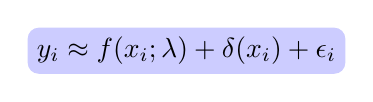
\begin{tikzpicture} \node [rounded corners,fill=blue!20] {
$y_i \approx f(x_i;\lambda)+\delta(x_i)+\epsilon_i$
};
\end{tikzpicture}
}
\bi
\item Difficult to distinguish contributions between model and data errors
\item No longer guarantees physical constraints in $g_i$
\item Unable to predict other QoIs with model error
\item Does not use \textit{a priori} knowledge of discrepancy structure
\ei

\vspace{1em}
%\item
\textbf{Our approach:} embedded model \mycit{S., Najm, Ghanem, 2015; S., Huan, Najm, 2018}

\centerline{$\qquad$
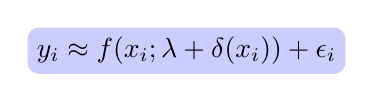
\begin{tikzpicture} \node [rounded corners,fill=blue!20] {
$y_i \approx f(x_i;\lambda+\delta(x_i))+\epsilon_i$
};
\end{tikzpicture}
}
\bi
\item Embeds model error in specific submodel phenomenology
\item Allows \textit{targeted} placement of model error term (e.g., in
  locations where key modeling assumptions and approximations are
  made)
\item Disambiguates model error from data noise
\item Inherits model structure and physical constraints
\ei
%\ei

\end{frame}
%==============================================================================
